\chapter{Overview of the hardware}

\section{Introduction}
The magnetometer is designed for low-power operation, simple
installation and ease of construction. 

The magnetometer has two parts, the interfacing unit, which is fitted
onto the Raspberry Pi's \gpio\ expansion header, and the sensor
head. Both parts are located indoors. This simplifies the installation
but makes the magnetometer very much more sensitive to temperature
variations and human disturbance. The sensor head should be located,
as much as as is practical, in an environment with stable temperature
control and away from major sources of human disturbance (particularly
cars and lifts).

\begin{figure}
  \centering
  \todo
  %%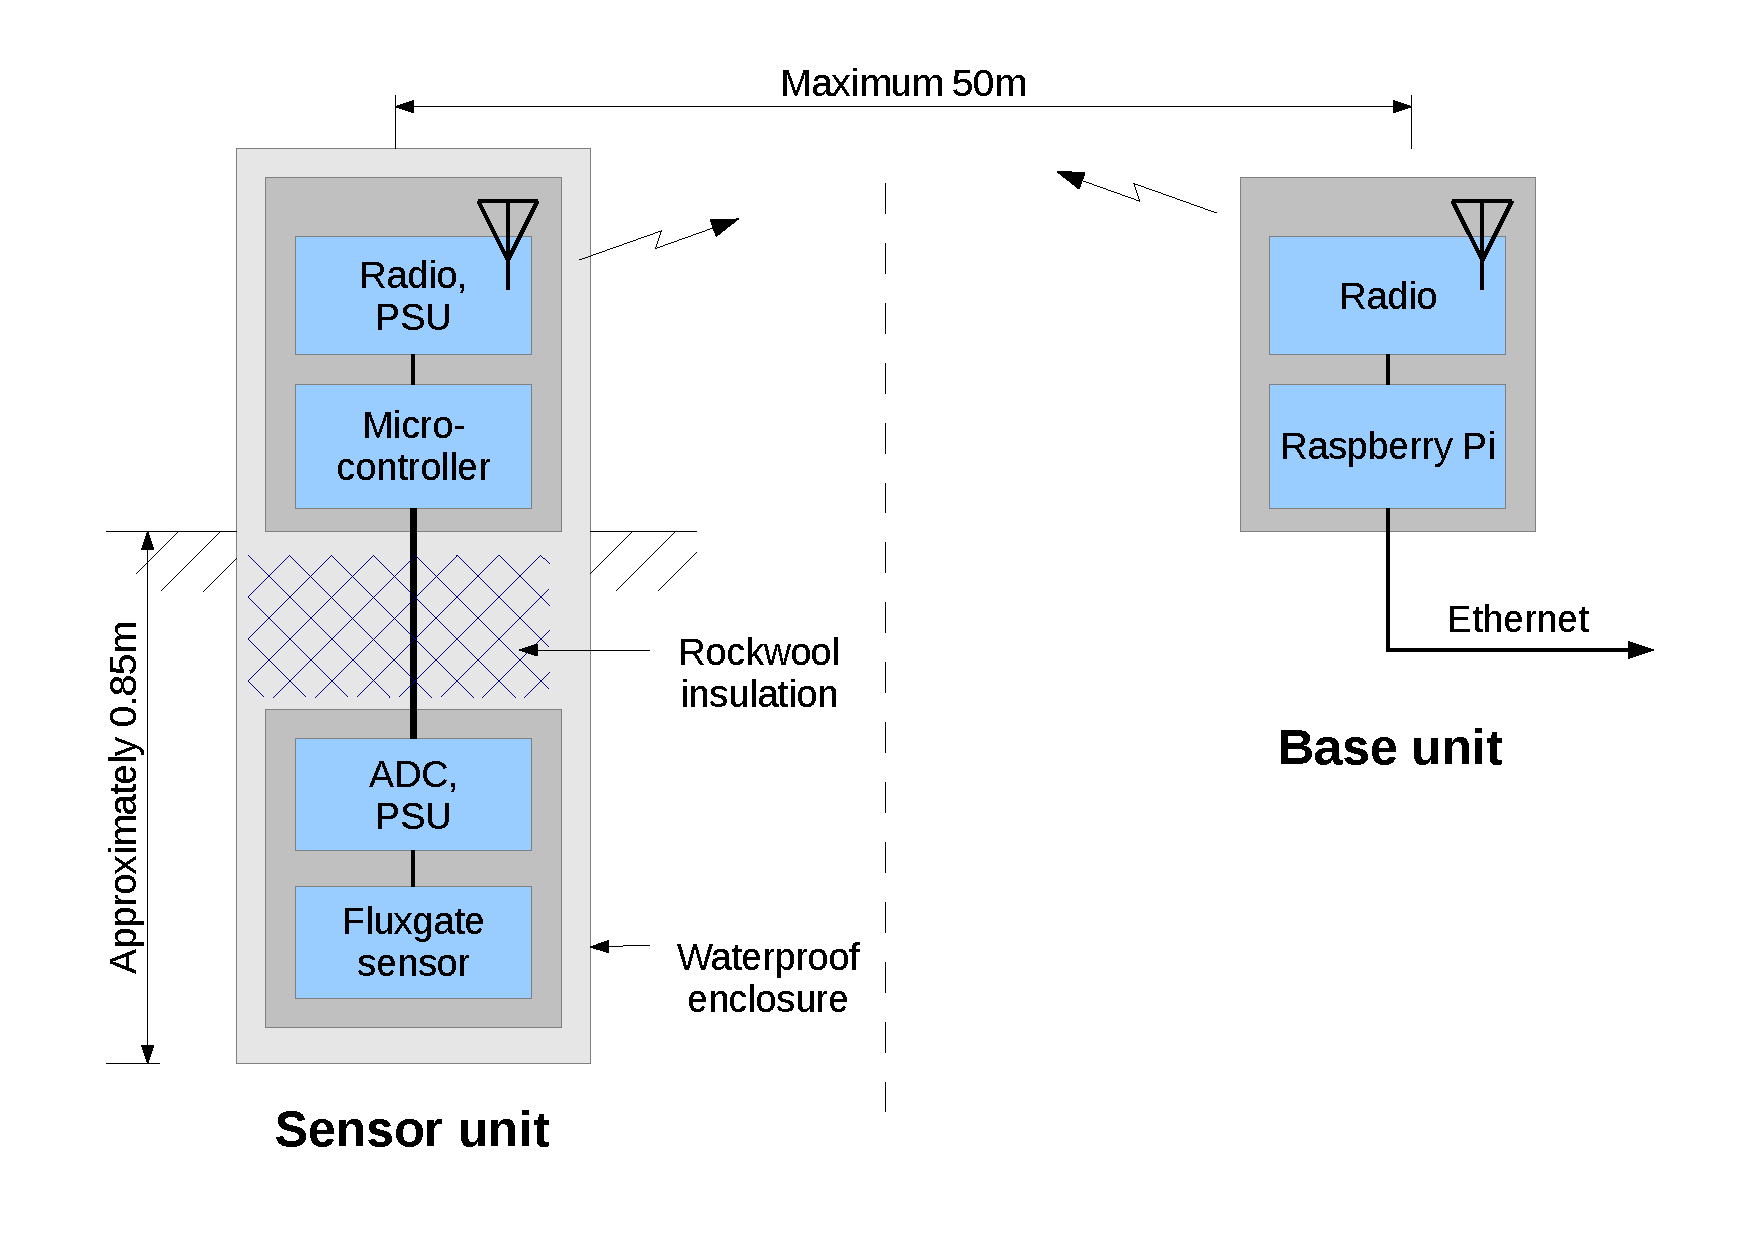
\includegraphics[keepaspectratio,width=\textwidth]{%
  %%  raspi-mag/images/system-overview}
  \caption[System overview]%
  {System overview.}
  \label{fig:system-overview}
\end{figure}

